\subsection*{Dataset and application context}
Click through rate prediction is one example of a large scale, temporally structured, tabular classification problem.
An advertisement is shown to a user in response to a page view or an app interaction.
Each showing is an impression.
Some impressions lead to a click.
The click through rate is the probability of click conditional on an impression.
Accurate click probability estimates are used in ranking and bidding pipelines.

The Avazu dataset is a public snapshot of an ad marketplace log at impression level.
Each row corresponds to one impression and includes a binary click label and a timestamp at hour resolution.
The feature space is dominated by high cardinality categorical identifiers that describe the user device, the application, and the site.
These identifiers induce strong repetition patterns and create a large cold start surface as new values appear over time.
The label is sparse, so PR AUC complements ROC AUC by emphasizing precision and recall under class imbalance.

This setting is temporally nonstationary.
Traffic composition and user intent change over time, and the statistical relationship between identifiers and click probability drifts.
Therefore, offline evaluation must be time aware.
This paper uses strict out of time splits and a no lookahead simulation of feature availability.
These constraints aim to prevent leakage and to better approximate a production deployment where features must be computed from past events only.

\subsection{Deterministic sampling procedure}
\label{sec:appendix_sampling}
The ten percent sample is constructed deterministically by applying a hash filter to the Avazu row identifier while streaming the dataset.
For each row, the identifier is hashed with the pandas function \texttt{hash\_pandas\_object} and interpreted as an unsigned 64-bit integer $h$.
The row is included in the ten percent sample if $(h \bmod 100) < 10$.
This procedure is deterministic within a fixed pandas version.
Pandas does not guarantee cross-version hash stability, so exact sample identity may change across pandas versions.

\subsection*{Model hyperparameters}
Table \ref{tab:xgb_params} reports XGBoost hyperparameters used in all experiments.

\begin{table}[t]
  \centering
  \begin{tabular}{ll}
    \toprule
    Hyperparameter & Value \\
    \midrule
    $n\_estimators$ & 800 \\
    $learning\_rate$ & 0.05 \\
    $max\_depth$ & 6 \\
    $subsample$ & 0.8 \\
    $colsample\_bytree$ & 0.8 \\
    $min\_child\_weight$ & 10.0 \\
    $reg\_lambda$ & 5.0 \\
    $random\_state$ & 42 \\
    $n\_jobs$ & 1 \\
    $tree\_method$ & \texttt{hist} \\
    \bottomrule
  \end{tabular}
  \caption{XGBoost hyperparameters used in all experiments.}
  \label{tab:xgb_params}
\end{table}

\subsection{Time-aware target encoding}
\label{sec:appendix_te_details}
This section specifies the target encoding baseline used in the paper.
Target encoding is computed at hour resolution with a one hour shift.
For a row at hour $h$, statistics use only labels from hours $< h$.

\subsubsection*{Split-boundary handling}
For each fold, target encoding and time aggregation features are computed for all rows in chronological order before slicing into train, validation, and test splits.
Therefore, features in the validation and test splits may depend on label feedback from earlier hours in the same fold, including earlier hours within the same day, but never from the current hour.
This matches a streaming evaluation setting in which click outcomes become available with one hour delay.

The model is trained on numeric features only.
It includes:
\begin{itemize}
  \item base time features: hour of day and the global prior $\mathrm{prior\_ctr}(h)$,
  \item for each categorical column $c$: a target encoding feature $c\_\_te$ and a history volume feature $c\_\_hist\_imps=\log(1+I_{v,<h})$.
\end{itemize}

Table \ref{tab:cat_cols} lists the categorical columns that are target encoded in the ten percent sample.

\begin{table}[t]
  \centering
  \small
  \begin{tabular}{lll}
    \toprule
    \multicolumn{3}{c}{Categorical columns} \\
    \midrule
    C1 & banner\_pos & site\_id \\
    site\_domain & site\_category & app\_id \\
    app\_domain & app\_category & device\_id \\
    device\_ip & device\_model & device\_type \\
    device\_conn\_type & C14 & C15 \\
    C16 & C17 & C18 \\
    C19 & C20 & C21 \\
    \bottomrule
  \end{tabular}
  \caption{Categorical columns target encoded in the ten percent sample.}
  \label{tab:cat_cols}
\end{table}

The global time-aware prior CTR is
\[
\mathrm{prior\_ctr}(h) = \frac{C_{<h} + a}{I_{<h} + a + b},
\]
with $a=1$ and $b=10$, where $I_{<h}$ and $C_{<h}$ are cumulative impressions and clicks over hours $< h$.

For a categorical column $c$ and value $v$, define cumulative counts $I_{v,<h}$ and $C_{v,<h}$ over hours $<h$.
The target encoding value is
\[
\mathrm{TE}_c(v,h) = \frac{C_{v,<h} + m \cdot \mathrm{prior\_ctr}(h)}{I_{v,<h} + m},
\]
with smoothing strength $m=100$.
If a value is unseen, $I_{v,<h}=0$ and the encoder returns $\mathrm{prior\_ctr}(h)$.
In this case, $c\_\_hist\_imps=\log(1+0)=0$.

The algorithm is deterministic and can be summarized as follows.
\begin{enumerate}
  \item Sort rows by hour in ascending order.
  \item For each hour $h$, compute $\mathrm{prior\_ctr}(h)$ from cumulative counts over hours $<h$.
  \item For each categorical column $c$ and each row at hour $h$ with value $v$, compute $c\_\_te$ and $c\_\_hist\_imps$ from $I_{v,<h}$ and $C_{v,<h}$.
  \item After processing hour $h$, update cumulative counts with all rows from hour $h$.
\end{enumerate}

\begin{figure}[t]
  \centering
  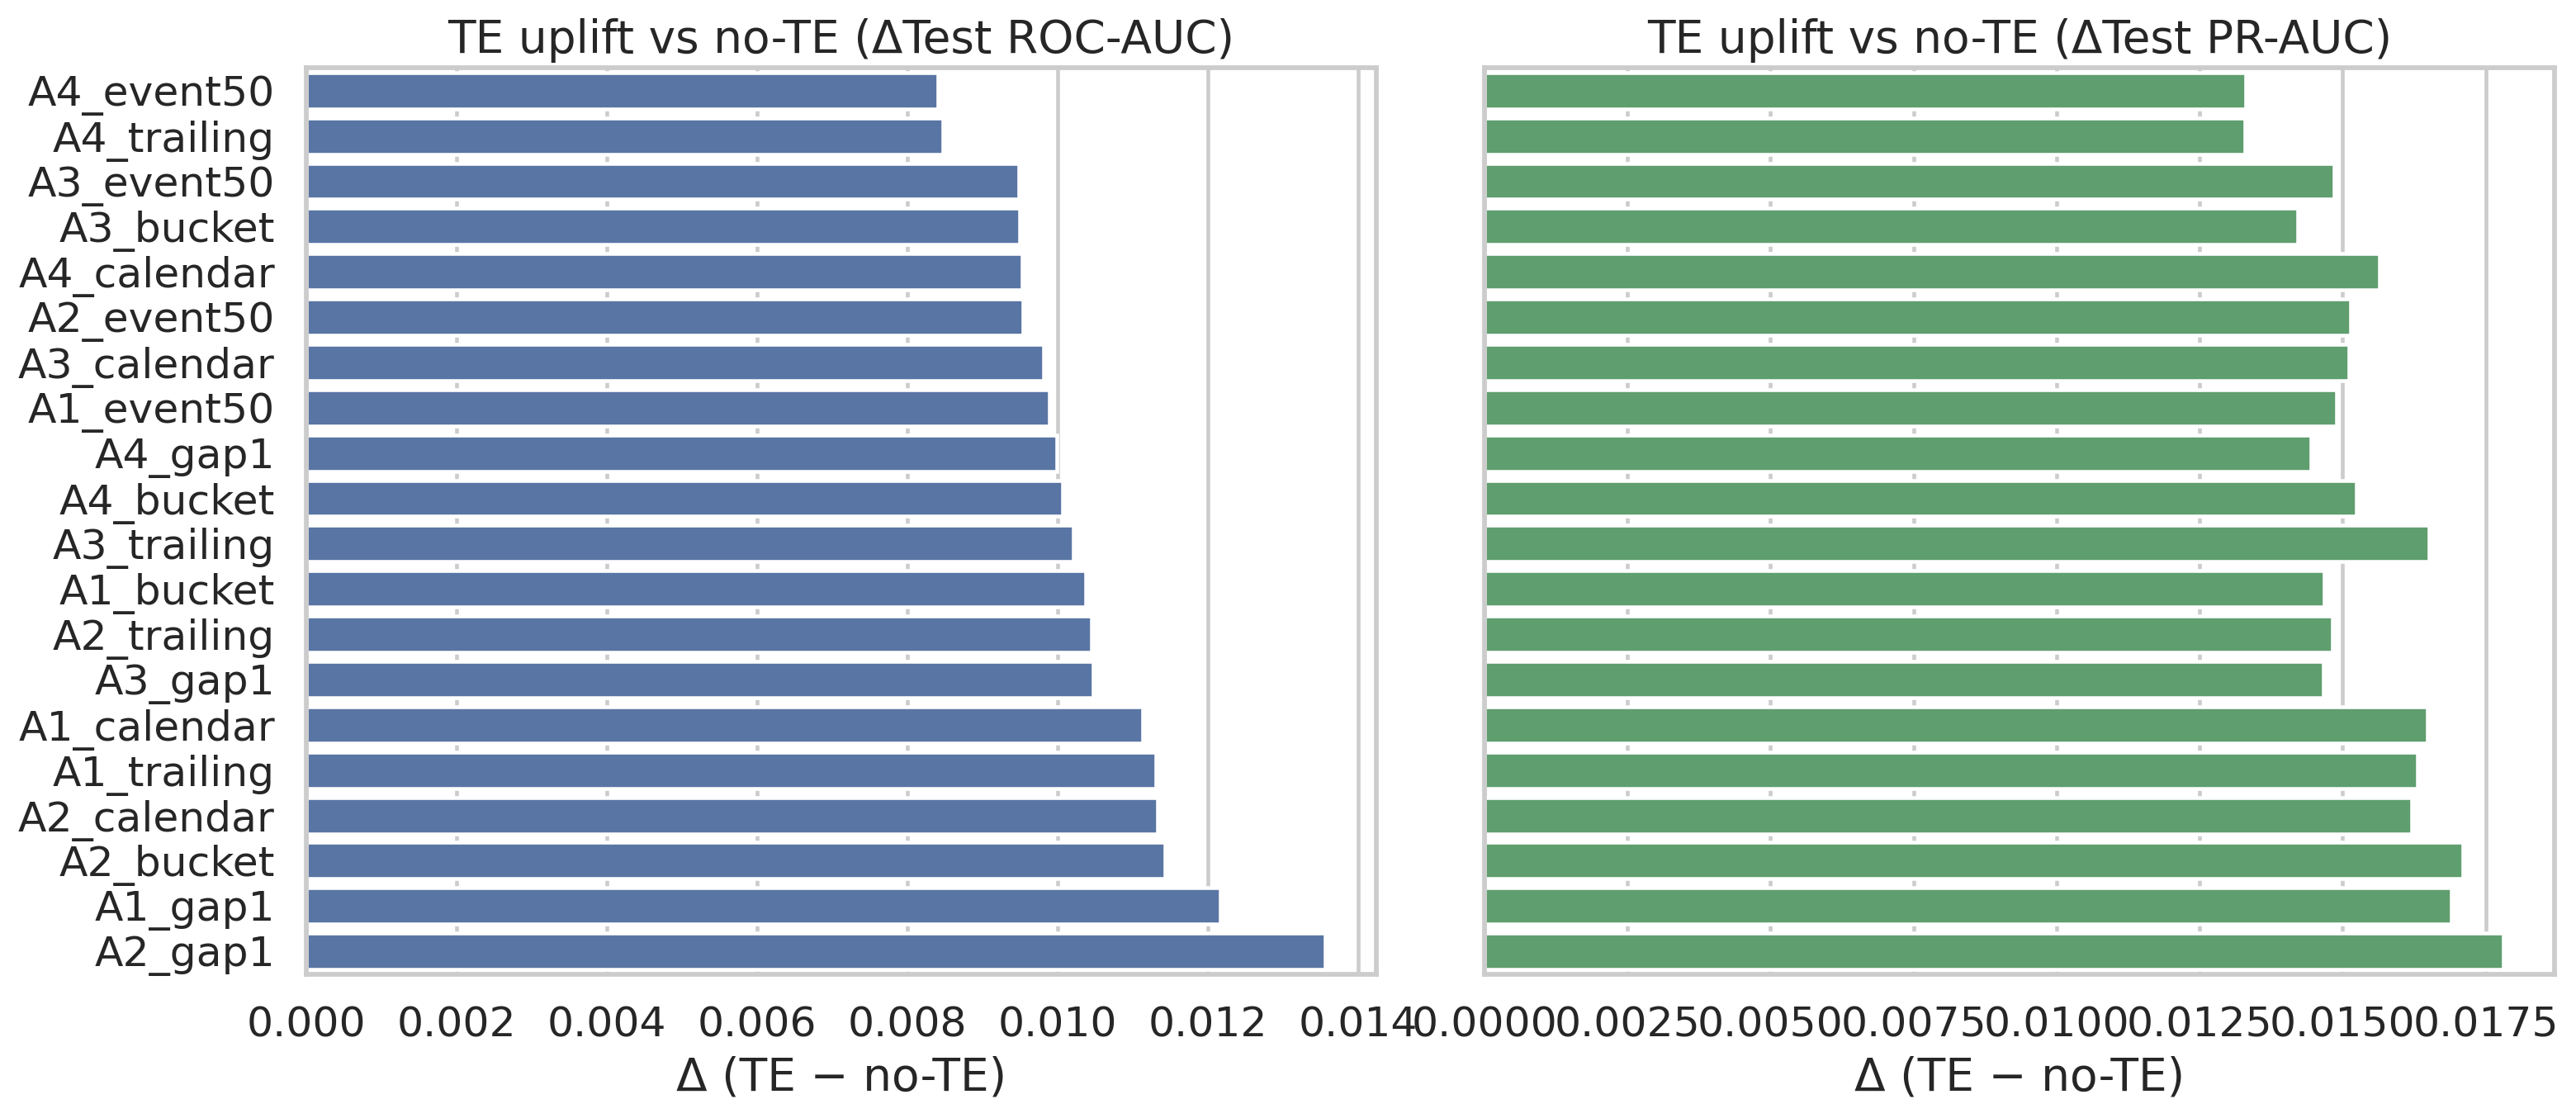
\includegraphics[width=\linewidth]{figures/te_vs_note_uplift.png}
  \caption{Uplift from adding target encoding on top of time aggregation features.}
  \label{fig:te_uplift}
\end{figure}

\subsection{Time aggregation feature definitions}
\label{sec:appendix_timeagg_defs}
Time aggregation features are computed online-safe with per-hour batching.
For a row at hour $h$, all entity-history statistics use only data from hours $<h$.
Each entity feature uses impression and click counts in a window, reported as $\log(1+I)$ and a smoothed rate $(C+\alpha)/(I+\alpha+\beta)$ with $\alpha=1$ and $\beta=10$.

\paragraph{Trailing windows.}
For entity column $e$ and entity value $v$, and window length $w$ hours, define impressions $I_{v,[h-w,h)}$ and clicks $C_{v,[h-w,h)}$ over $[h-w,h)$.
The features are $\log(1+I_{v,[h-w,h)})$ and $(C_{v,[h-w,h)}+\alpha)/(I_{v,[h-w,h)}+\alpha+\beta)$.

\paragraph{Gap windows.}
For gap size $g$, define $[h-w-g,h-g)$ and compute counts as differences of trailing windows.

\paragraph{Bucket windows.}
Given edges $0<b_1<\dots<b_K$, bucket $j$ is $[h-b_j,h-b_{j-1})$ with $b_0=0$.
Counts are computed as differences of trailing windows at horizons $b_j$ and $b_{j-1}$.

\paragraph{Calendar windows.}
Calendar features include counts and smoothed rates for the current day up to hour $h$ and, when available, for the previous day.

\paragraph{Recency.}
For each entity value, recency is the time since last observation in hours.
Recency is undefined for unseen entities and is represented as NaN.

\paragraph{Event-count window.}
For each entity value, the event-count window uses the most recent $N$ impressions strictly before hour $h$.
When an entity has fewer than $N$ prior impressions, the features are computed from its available history, and the $\alpha,\beta$ smoothing prevents extreme rates.
In this paper, the event-count shape uses $N=50$.

\subsection{Feature dimensionality}
\label{sec:appendix_feature_dimensionality}
Table \ref{tab:feature_counts} reports total feature counts for each length tuple and shape in the target encoding grid.

\begin{table}[t]
  \centering
  \small
  \begin{tabular}{llr}
\toprule
Length tuple (hours) & Shape & Total features \\
\midrule
$(1, 6, 24)$ & trailing & 72 \\
$(1, 6, 24)$ & gap1 & 72 \\
$(1, 6, 24)$ & bucket & 72 \\
$(1, 6, 24)$ & calendar & 88 \\
$(1, 6, 24)$ & event50 & 80 \\
$(1, 3, 6, 12, 24)$ & trailing & 88 \\
$(1, 3, 6, 12, 24)$ & gap1 & 88 \\
$(1, 3, 6, 12, 24)$ & bucket & 88 \\
$(1, 3, 6, 12, 24)$ & calendar & 104 \\
$(1, 3, 6, 12, 24)$ & event50 & 96 \\
$(1, 6, 24, 48, 168)$ & trailing & 88 \\
$(1, 6, 24, 48, 168)$ & gap1 & 88 \\
$(1, 6, 24, 48, 168)$ & bucket & 88 \\
$(1, 6, 24, 48, 168)$ & calendar & 104 \\
$(1, 6, 24, 48, 168)$ & event50 & 96 \\
$(1, 2, 4, 8, 16, 24, 48, 96, 168)$ & trailing & 120 \\
$(1, 2, 4, 8, 16, 24, 48, 96, 168)$ & gap1 & 120 \\
$(1, 2, 4, 8, 16, 24, 48, 96, 168)$ & bucket & 120 \\
$(1, 2, 4, 8, 16, 24, 48, 96, 168)$ & calendar & 136 \\
$(1, 2, 4, 8, 16, 24, 48, 96, 168)$ & event50 & 128 \\
\bottomrule
\end{tabular}

  \caption{Total number of model input features for each window specification in the target encoding plus time aggregation grid.}
  \label{tab:feature_counts}
\end{table}

\subsection{Additional absolute metrics}
\label{sec:appendix_top_specs_absolute_metrics}
Table \ref{tab:top_specs_absolute} reports absolute test metrics for representative high-performing specifications in the target encoding plus time aggregation grid.

\begin{table}[t]
  \centering
  \small
  \resizebox{\linewidth}{!}{%
  \begin{tabular}{llcccc}
\toprule
Length tuple (hours) & Shape & Test ROC AUC A & Test ROC AUC B & Test PR AUC A & Test PR AUC B \\
\midrule
$(1, 6, 24)$ & event50 & 0.7486 & 0.7522 & 0.3774 & 0.3576 \\
$(1, 3, 6, 12, 24)$ & calendar & 0.7478 & 0.7516 & 0.3766 & 0.3566 \\
$(1, 3, 6, 12, 24)$ & event50 & 0.7484 & 0.7522 & 0.3788 & 0.3571 \\
$(1, 6, 24, 48, 168)$ & calendar & 0.7483 & 0.7518 & 0.3774 & 0.3564 \\
$(1, 6, 24, 48, 168)$ & event50 & 0.7486 & 0.7524 & 0.3784 & 0.3574 \\
$(1, 6, 24, 48, 168)$ & trailing & 0.7483 & 0.7520 & 0.3787 & 0.3563 \\
$(1, 2, 4, 8, 16, 24, 48, 96, 168)$ & calendar & 0.7473 & 0.7519 & 0.3772 & 0.3562 \\
$(1, 2, 4, 8, 16, 24, 48, 96, 168)$ & event50 & 0.7475 & 0.7517 & 0.3769 & 0.3560 \\
\bottomrule
\end{tabular}

  }
  \caption{Absolute test metrics for selected high-performing specifications. Values are reported separately for Fold A and Fold B on the ten percent sample.}
  \label{tab:top_specs_absolute}
\end{table}

\subsection{Compute considerations}
\label{sec:appendix_compute}
The ten percent sample contains about 4.04 million rows.
In the sweep driver logs, the subset of runs that executed in that invocation took 13.9 to 21.2 minutes wall time per run with $n\_jobs=1$.
The same logs recorded a minimum available RAM of 6.45 GiB and minimum free swap of 5.57 GiB during execution.

Target encoding can be computed on the fly from the raw dataset, but this is expensive because it requires repeated hour-shifted aggregations per categorical column.
For the ten percent grid, target encoding features are precomputed and cached in a parquet to amortize this cost.
With target encoding cached, feature generation runtime is dominated by the time aggregation streaming pass and by materializing the dense float32 training matrix for millions of rows.
Peak memory is dominated by large in-memory arrays for the feature matrix and intermediate frames, with additional overhead from per-entity history state.

\subsection{Event-count window sensitivity}
\label{sec:appendix_event_count_sensitivity}
Figure \ref{fig:event_count_sweep} reports a small sensitivity sweep that varies the event-count window size $N$ on a one percent sample with target encoding enabled and length tuple $(1, 6, 24, 48, 168)$.
This sweep uses a single split rather than the rolling tail protocol.

\begin{figure}[t]
  \centering
  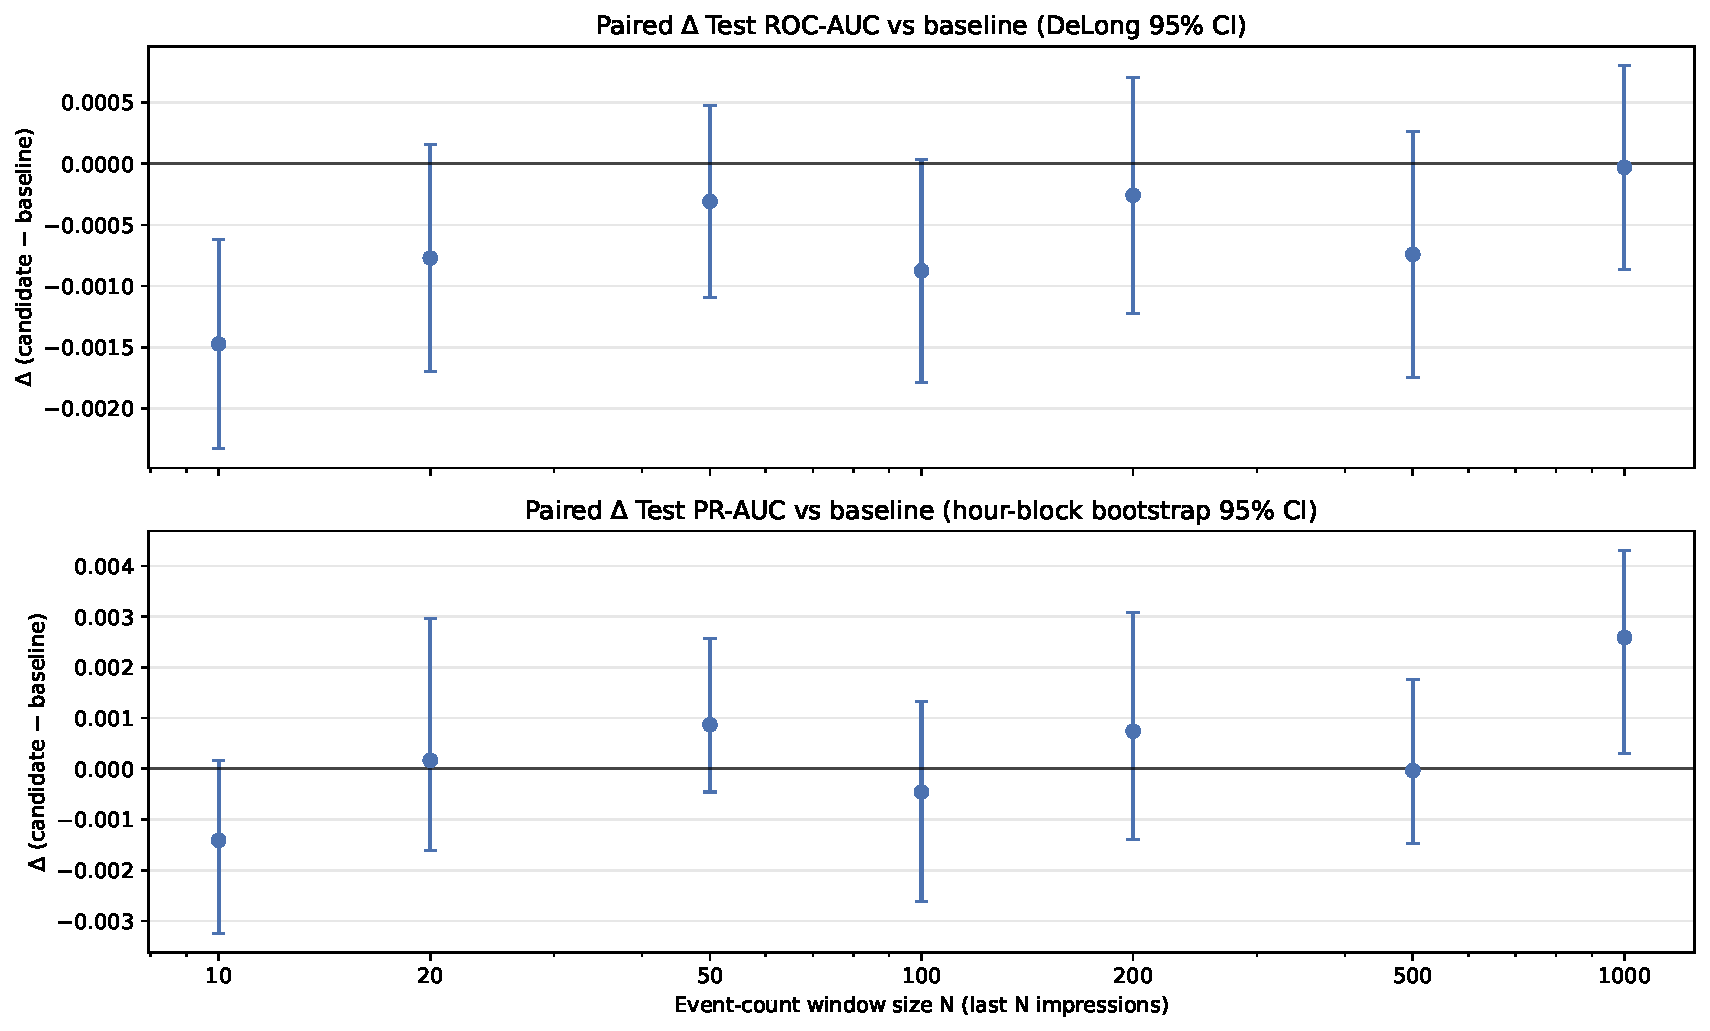
\includegraphics[width=\linewidth]{figures/fig_event_count_sweep_1pct.pdf}
  \caption{Sensitivity of event-count window size $N$ on a one percent sample with target encoding and length tuple $(1, 6, 24, 48, 168)$. Performance is relatively flat across a wide range of $N$ in this single-split experiment.}
  \label{fig:event_count_sweep}
\end{figure}

\subsection*{EDA context}
Figure \ref{fig:eda_ctr} shows CTR drift by day.
Figure \ref{fig:eda_unseen} shows an unseen rate summary for top categorical features.
These plots provide context for why out of time evaluation and cold start effects matter.

\begin{figure}[t]
  \centering
  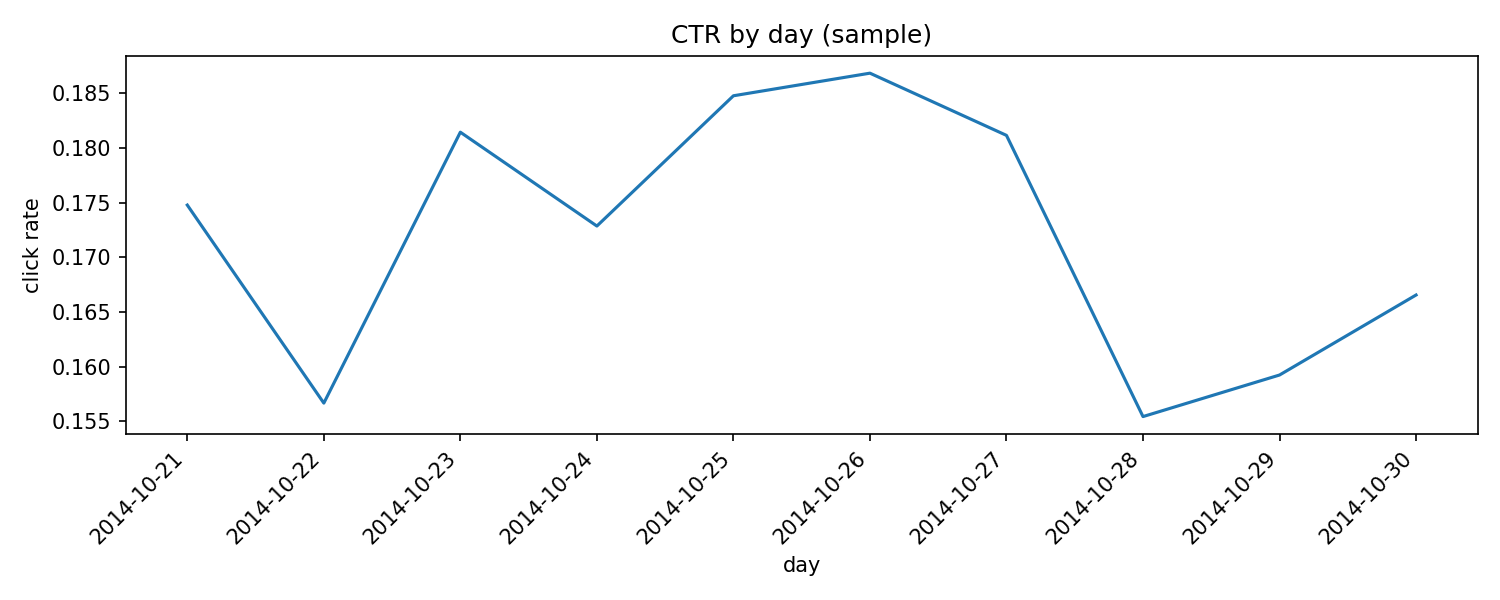
\includegraphics[width=\linewidth]{figures/eda_ctr_by_day.png}
  \caption{CTR by day in the dataset sample.}
  \label{fig:eda_ctr}
\end{figure}

\begin{figure}[t]
  \centering
  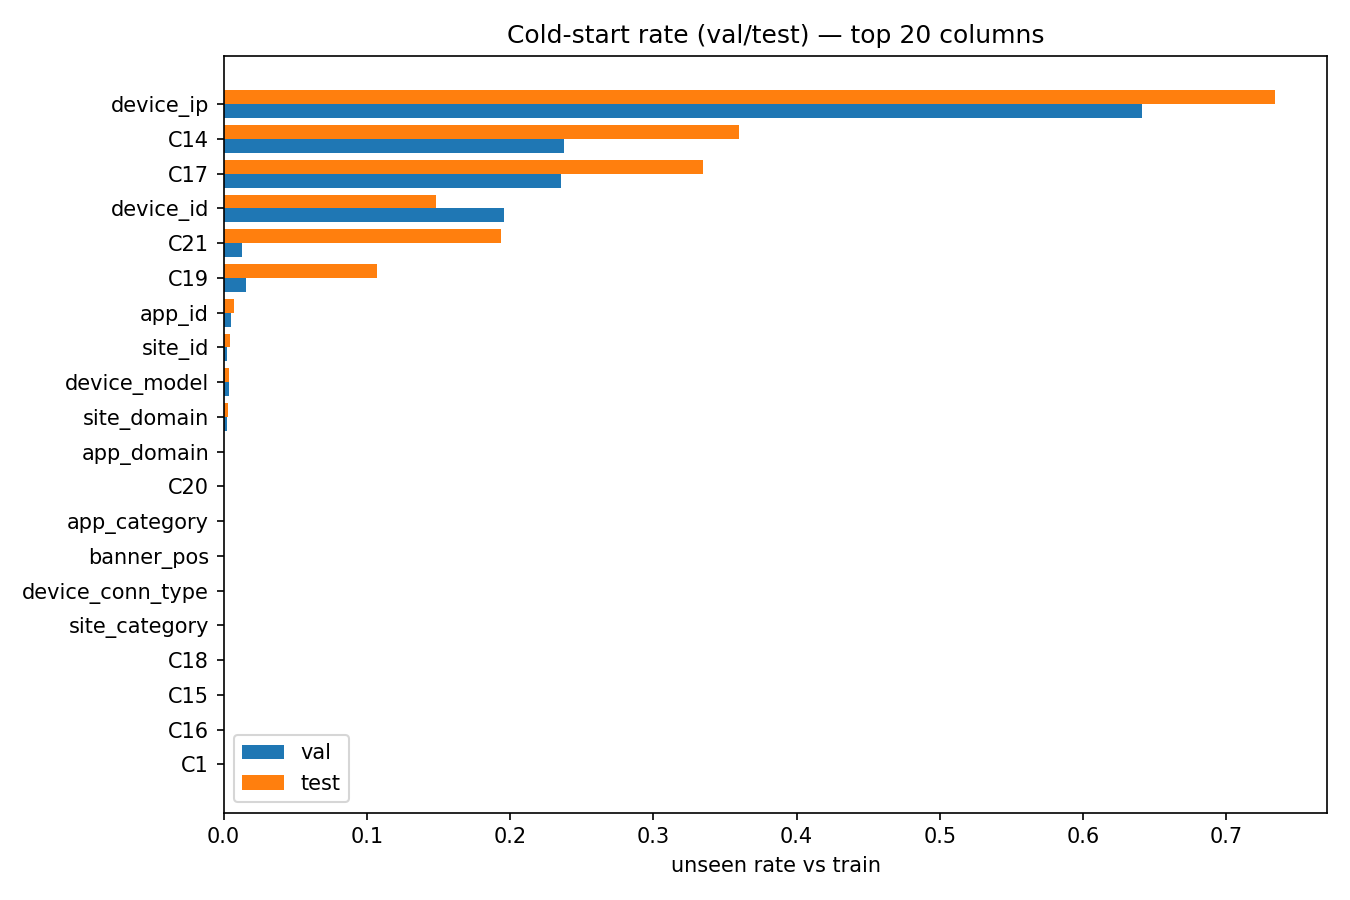
\includegraphics[width=\linewidth]{figures/eda_unseen_rate_top.png}
  \caption{Unseen rate for top categorical features across time.}
  \label{fig:eda_unseen}
\end{figure}

\subsection*{Full result tables}
This paper includes supplementary tables that report the full design grids and paired inference results.

\begin{figure}[t]
  \centering
  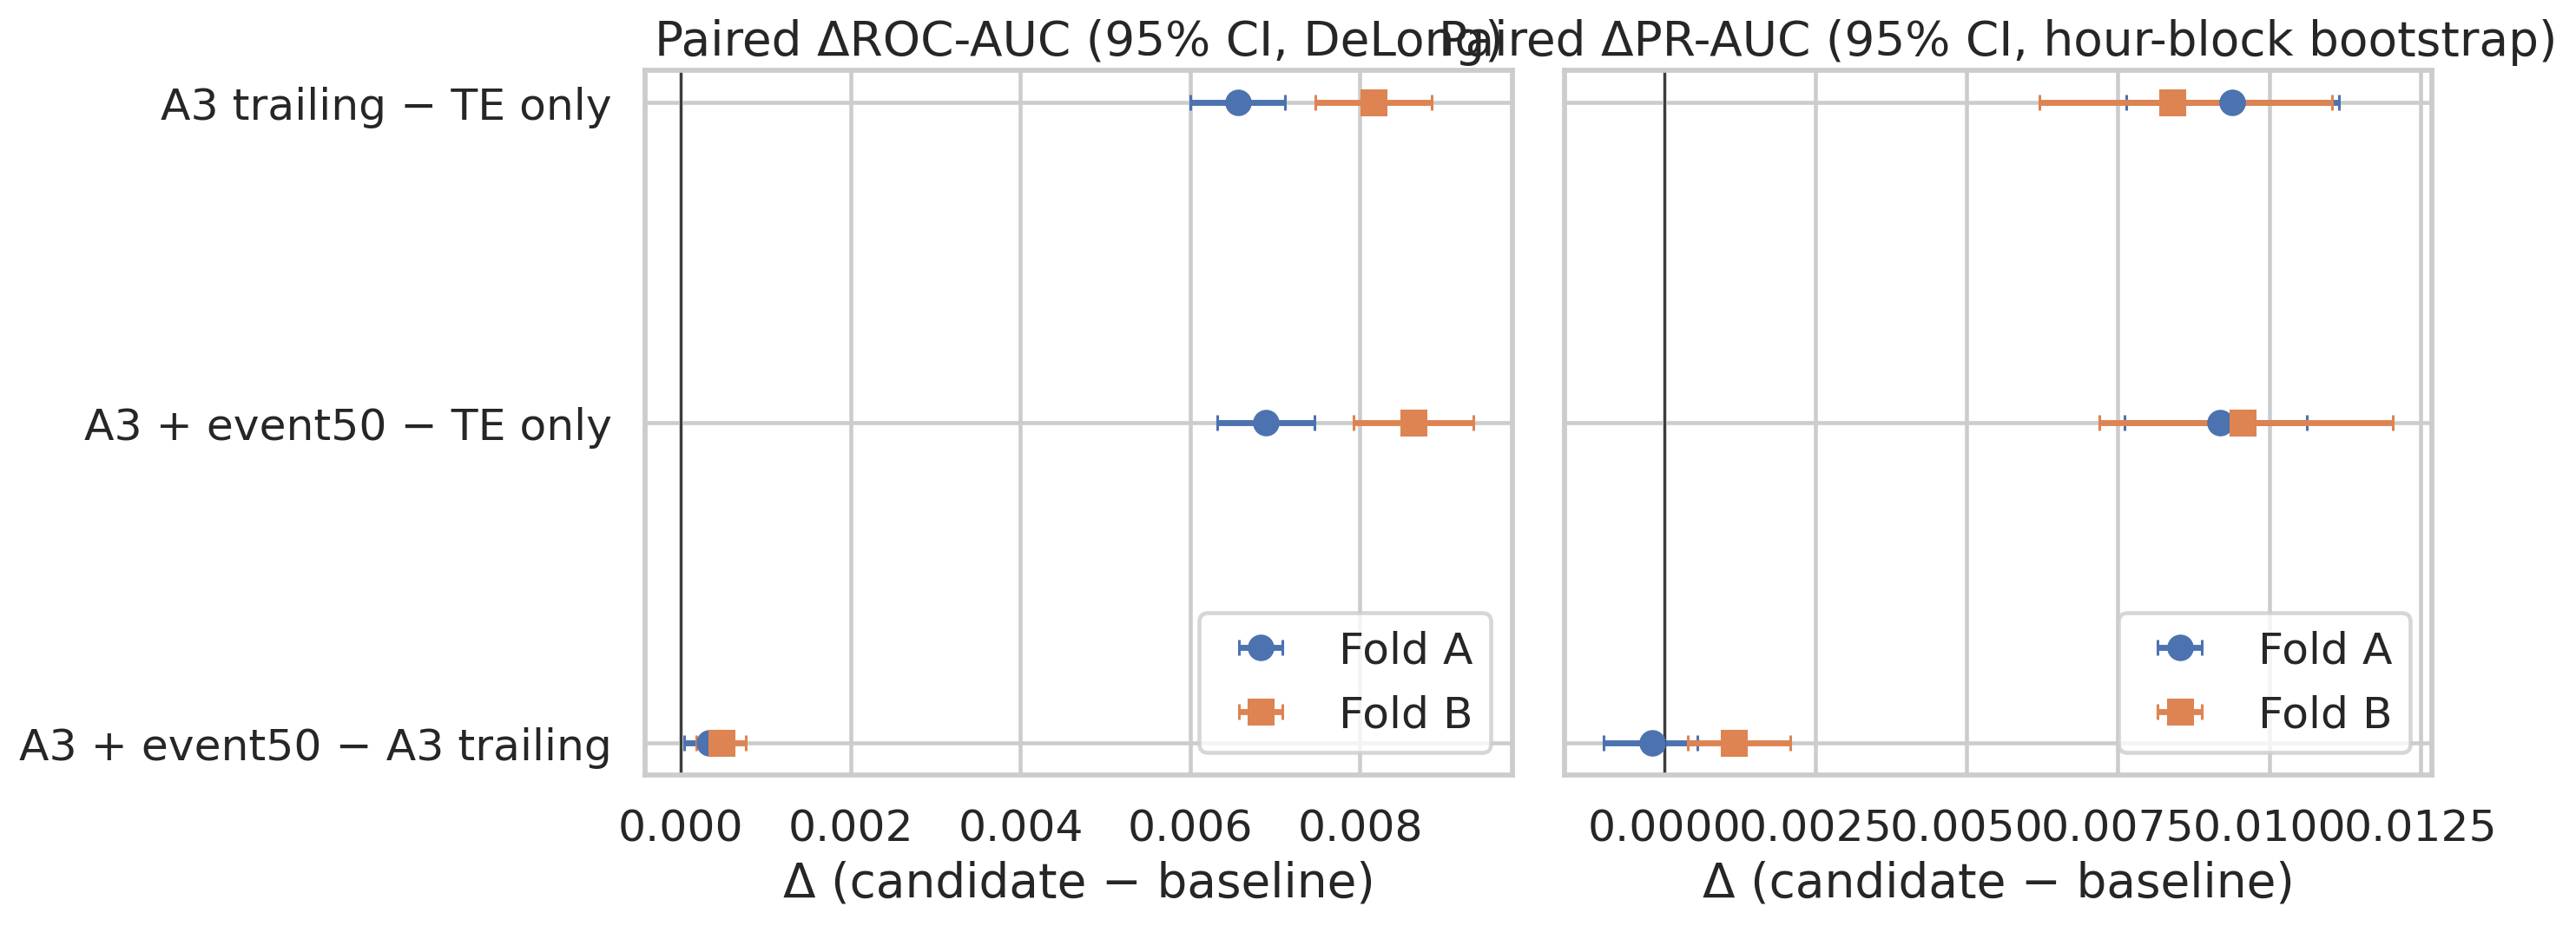
\includegraphics[width=0.92\linewidth]{figures/te_lift_deltas.png}
  \caption{Paired lift from adding time aggregation to a target encoding baseline under no lookahead evaluation.}
  \label{fig:te_lift_deltas}
\end{figure}

\begin{figure}[t]
  \centering
  
\includegraphics[width=\linewidth]{figures/fig_decision_lengths_then_shapes.pdf}
  \caption{Detailed view of length and shape effects with paired deltas and fold specific estimates.}
  \label{fig:decision_plot}
\end{figure}
